\documentclass[12pt,a4paper]{article}
\usepackage[margin=25mm]{geometry}
\usepackage[T1]{fontenc}
\usepackage[utf8]{inputenc}
\usepackage{lmodern}
\usepackage{graphicx}
\usepackage{amsmath,amssymb}
\usepackage{booktabs}
\usepackage{tabularx}
\usepackage{float}
\usepackage{subcaption}
\usepackage{hyperref}
\usepackage{fancyhdr}
\usepackage{titlesec}

\graphicspath{{./}{figures/}{WhatsApp Unknown 2026-09-12 at 18.51.55/}}
\hypersetup{colorlinks=true,linkcolor=black,urlcolor=blue}
\pagestyle{fancy}
\fancyhf{}
\lhead{Biomechanics}
\rhead{EMG Practical}
\cfoot{\thepage}
\setlength{\headheight}{15pt}
\titleformat{\section}{\Large\bfseries}{\thesection}{0.7em}{}
\titleformat{\subsection}{\large\bfseries}{\thesubsection}{0.7em}{}
\newcommand{\csvfile}[1]{\texttt{\detokenize{#1}}}

\begin{document}

\begin{titlepage}
  \centering
  \vspace*{7mm}
  
\includegraphics[width=4.2cm]{campus_logo.png}\par\vspace{7mm}
  {\Large\bfseries Department of Electronic and Telecommunication Engineering\par}
  \vspace{2mm}{\large University of Moratuwa\par}
  \vspace{18mm}{\large B.Sc. Engineering\par}
  \vspace{5mm}{\Large\bfseries Biomechanics\par}
  \vspace{15mm}{\Huge\bfseries EMG Practical Report\par}
  \vspace{5mm}{\LARGE Raw EMG, RMS Feature Extraction, and MVC Normalisation\par}
  \vfill
  \renewcommand{\arraystretch}{1.35}
  \begin{tabular}{rl}
    \textbf{Laboratory:} & Biomechanics Laboratory \\
    \textbf{Assignment:} & Electromyography signal acquisition and interpretation \\
    \textbf{Student registration:} & 230449N \\
    \textbf{Data channel:} & EMG sensor 4, Channel 4 \\
    \textbf{Sampling frequency:} & $4000\,\mathrm{Hz}$ \\
  \end{tabular}
  \vfill
  {\large \today\par}
\end{titlepage}

\tableofcontents
\newpage

\section{Introduction}
Electromyography (EMG) measures the electrical activity generated by skeletal
muscle fibres during activation. Surface EMG is useful in biomechanics because
it provides a non-invasive estimate of muscle timing, relative effort, fatigue
effects, and differences between repeated movements or subjects. The recorded
signal is normally bipolar and noisy, so interpretation is improved by signal
processing steps such as rectification, root mean square (RMS) smoothing, and
normalisation to a maximum voluntary contraction (MVC).

The objective of this practical was to acquire raw EMG signals, extract RMS
features, record an MVC reference signal, and express the activity level of the
movement trials relative to the MVC. The available data files are organised as
raw trial recordings and an MVC sliding-RMS recording so that raw, RMS, and
normalised views can be compared.

\section{Methods}
\subsection{Apparatus}
The experiment used a surface EMG sensor connected to an acquisition system,
self-adhesive surface electrodes, a computer-based data capture interface, and
software capable of exporting comma-separated data. The exported files indicate
EMG sensor 4, Channel 4, with a sampling frequency of $4000\,\mathrm{Hz}$ and
voltage units.

\subsection{Electrode placement}
The skin over the target muscle was prepared before electrode attachment to
reduce contact impedance and motion artefact. The active electrodes were placed
over the muscle belly and aligned with the dominant fibre direction. A reference
electrode was attached to an electrically quiet bony area. The cable was secured
so that movement of the wire did not introduce avoidable artefacts into the
recording.

\subsection{Subject instruction and safety}
The subject was instructed to perform the selected motion consistently for each
trial and to avoid unnecessary body movement. For MVC acquisition, the subject
performed a brief maximum voluntary contraction against resistance. Rest periods
were allowed between efforts to reduce fatigue. The activity was stopped if pain
or discomfort occurred.

\subsection{Acquisition parameters}
\begin{table}[H]\centering
\caption{Data files used in the report.}
\begin{tabularx}{\textwidth}{lXr}
\toprule
\textbf{File} & \textbf{Signal content} & \textbf{Nominal samples} \\
\midrule
\csvfile{emg_raw_trial_16.csv} & Raw EMG movement trial labelled 16 & 82000 \\
\csvfile{emg_raw_trial_19.csv} & Raw EMG movement trial labelled 19 & 82000 \\
\csvfile{emg_raw_trial_27.csv} & Raw EMG movement trial labelled 27 & 8000 \\
\csvfile{emg_raw_trial_38.csv} & Raw EMG movement trial labelled 38 & 82000 \\
\csvfile{emg_mvc_sliding_rms.csv} & MVC signal after sliding RMS filtering & 110000 \\
\bottomrule
\end{tabularx}
\label{tab:data-files}
\end{table}

\subsection{Signal processing}
The raw EMG signal $x[n]$ was inspected to identify activation bursts and
artefacts. RMS processing was used because it gives a local estimate of signal
power while preserving the timing envelope of muscle activation:
\begin{equation}
 \mathrm{RMS}[n]=\sqrt{\frac{1}{N}\sum_{k=0}^{N-1}x^2[n-k]}.
\end{equation}
The RMS window should be long enough to smooth high-frequency oscillations but
short enough to retain changes in muscle activation. In this report the
interactive companion page allows the RMS window to be changed so the effect of
window length can be observed directly.

Amplitude normalisation was performed using the MVC reference:
\begin{equation}
 \%MVC[n]=\frac{\mathrm{RMS}_{trial}[n]}{\max(\mathrm{RMS}_{MVC})}\times100.
\end{equation}
This converts each trial into a relative activation level and makes comparisons
less dependent on electrode contact, sensor gain, and individual signal
amplitude.

\section{Results}

\subsection{Raw EMG}
The raw EMG recordings contain the original voltage-time signal from the sensor.
This graph is used to inspect signal quality, baseline noise, sudden motion
artefacts, clipping, and the timing of muscle activation. Raw EMG should not be
used alone for comparing effort because its high-frequency oscillations make
amplitude interpretation difficult.
\begin{figure}[H]\centering
 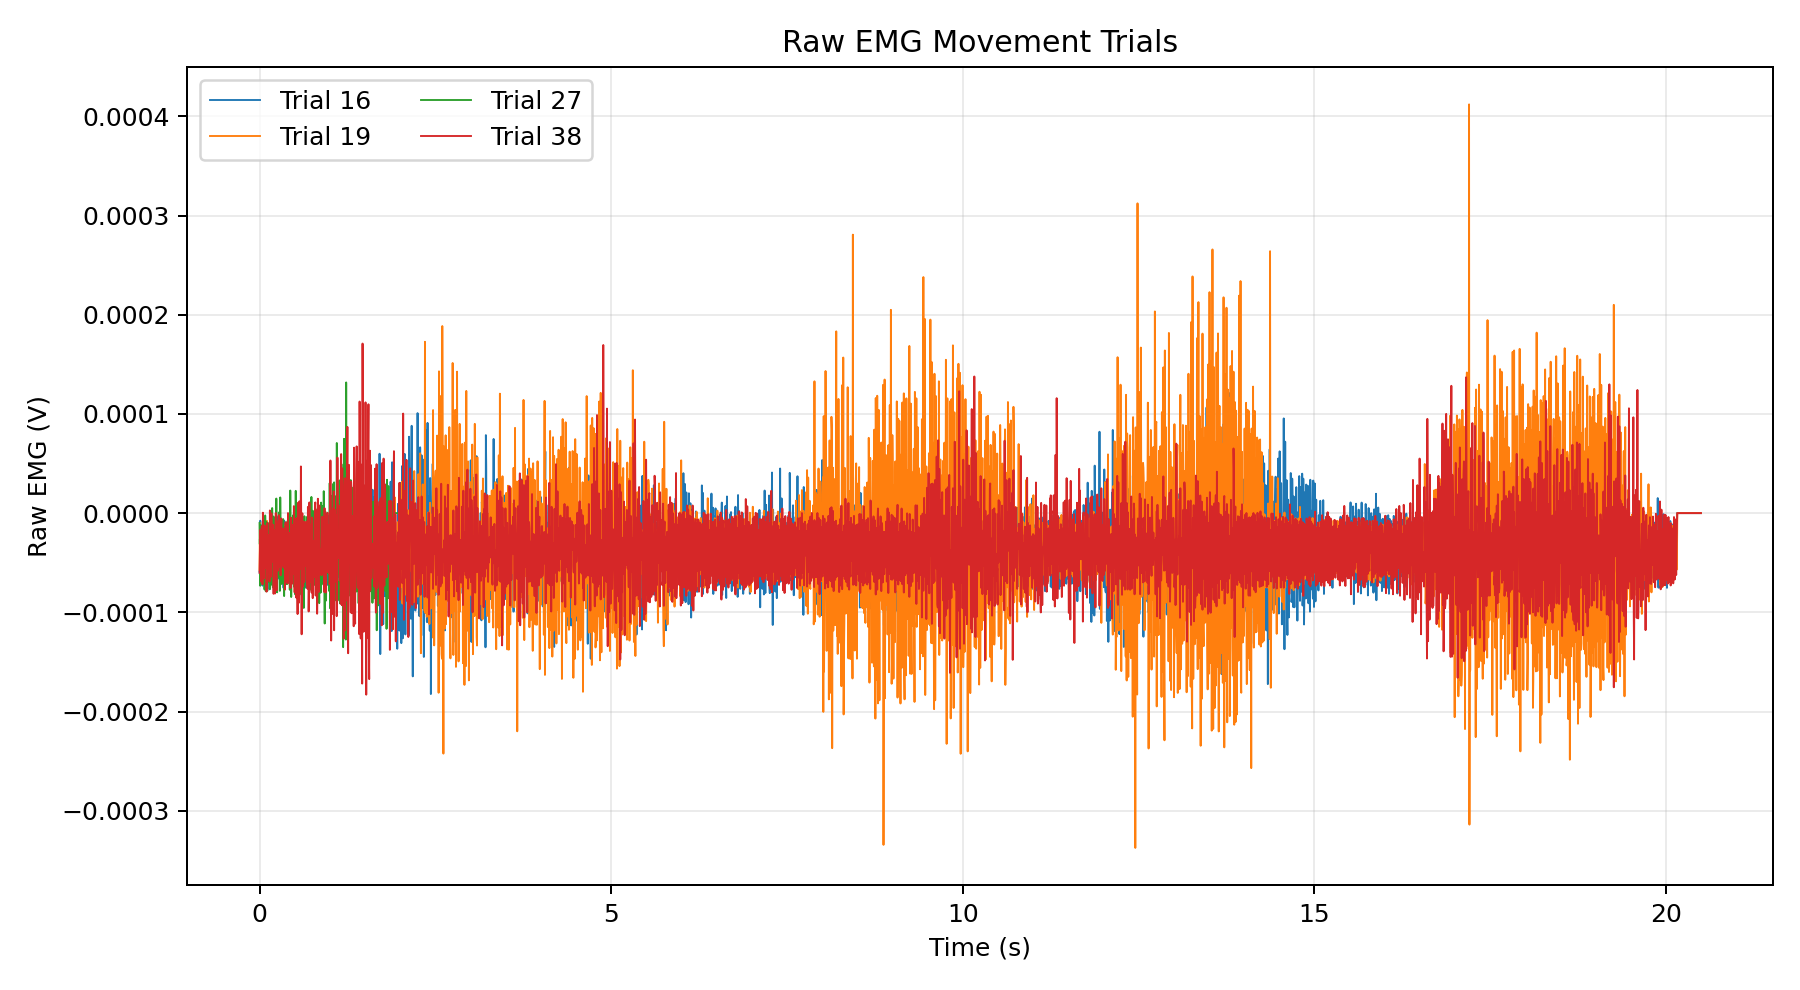
\includegraphics[width=0.95\textwidth]{emg_raw_trials.png}
 \caption{Raw EMG voltage traces for the four movement trials.}
 \label{fig:raw-emg}
\end{figure}

\subsection{RMS envelope}
The RMS graph is used as an activation envelope. It reduces the visual
complexity of the raw waveform and provides a feature proportional to local
signal energy. RMS values are suitable for comparing activation timing and
relative effort across repeated movements when the same processing window is
used.
\begin{figure}[H]\centering
 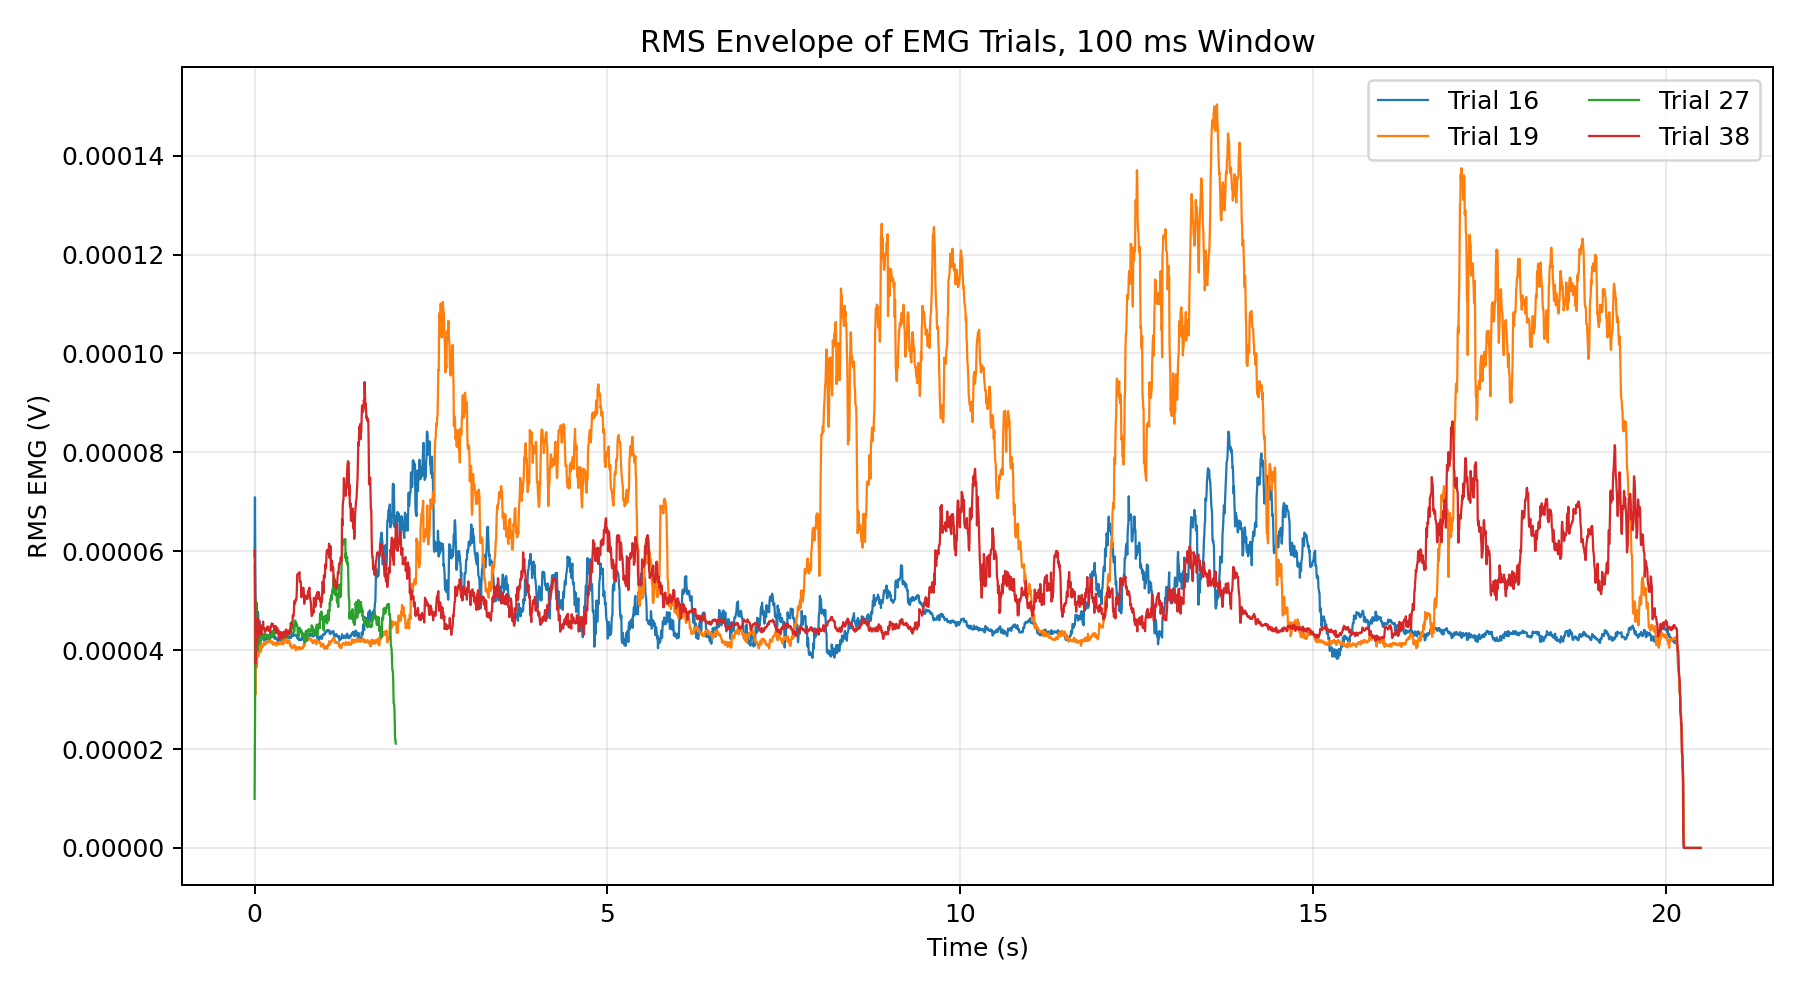
\includegraphics[width=0.95\textwidth]{emg_rms_trials.png}
 \caption{RMS envelopes computed from the raw EMG trials using a 100 ms moving window.}
 \label{fig:rms-emg}
\end{figure}

\subsection{MVC-normalised amplitude}
The MVC-normalised graph expresses trial activity as a percentage of the
maximum voluntary contraction reference. This graph is used to compare effort
between trials and subjects because it reports activity relative to a reference
capacity rather than in raw volts. In the data set, \csvfile{emg_mvc_sliding_rms.csv}
provides the MVC reference signal.
\begin{figure}[H]\centering
 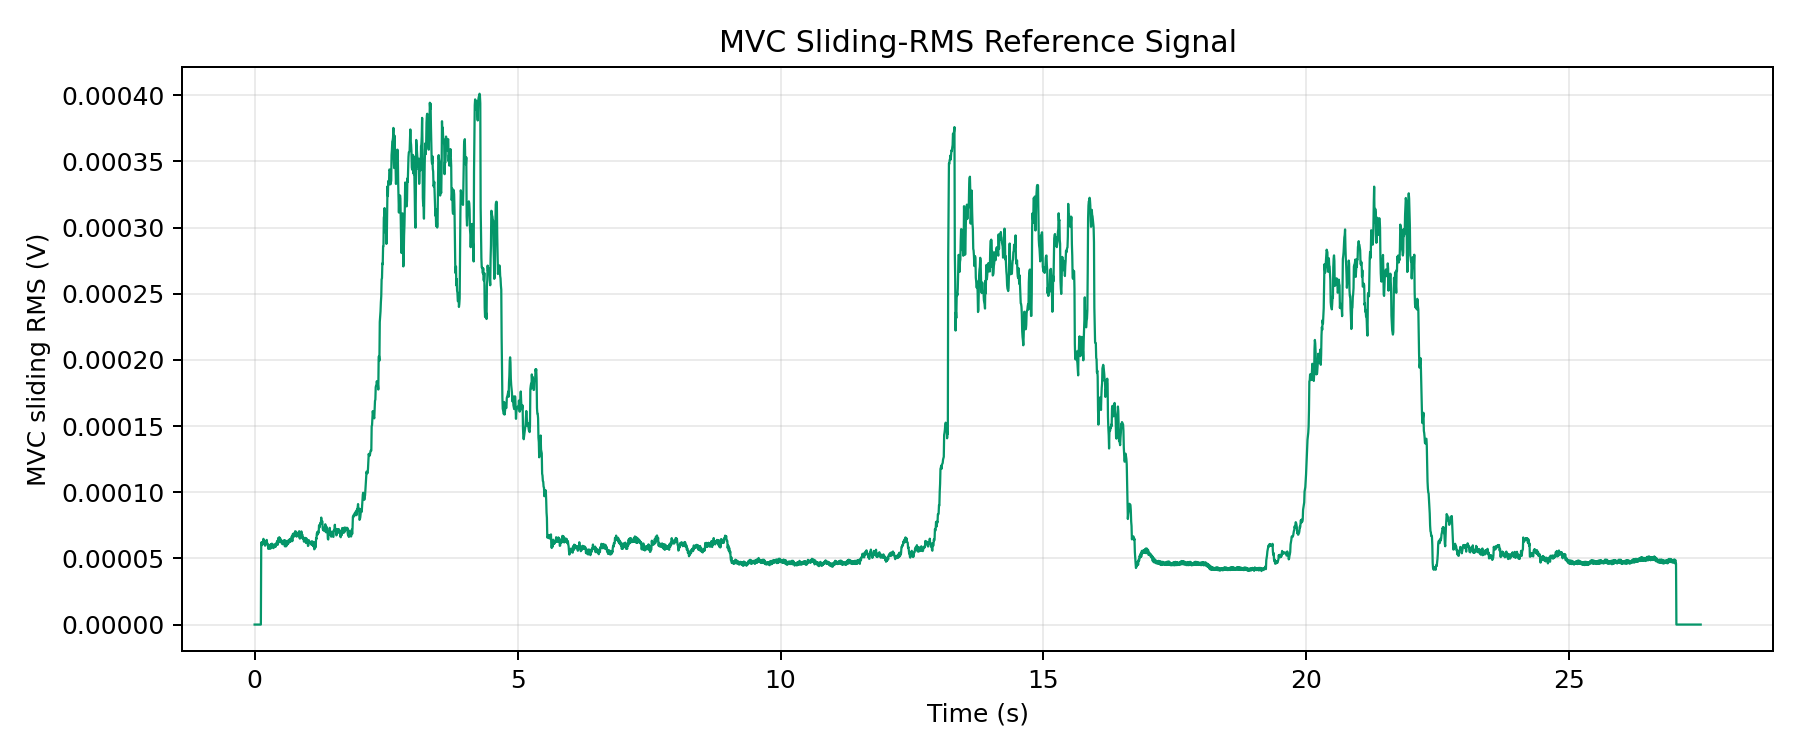
\includegraphics[width=0.95\textwidth]{emg_mvc_reference.png}
 \caption{MVC sliding-RMS reference used to normalise the movement-trial RMS envelopes.}
 \label{fig:mvc-reference}
\end{figure}
\begin{figure}[H]\centering
 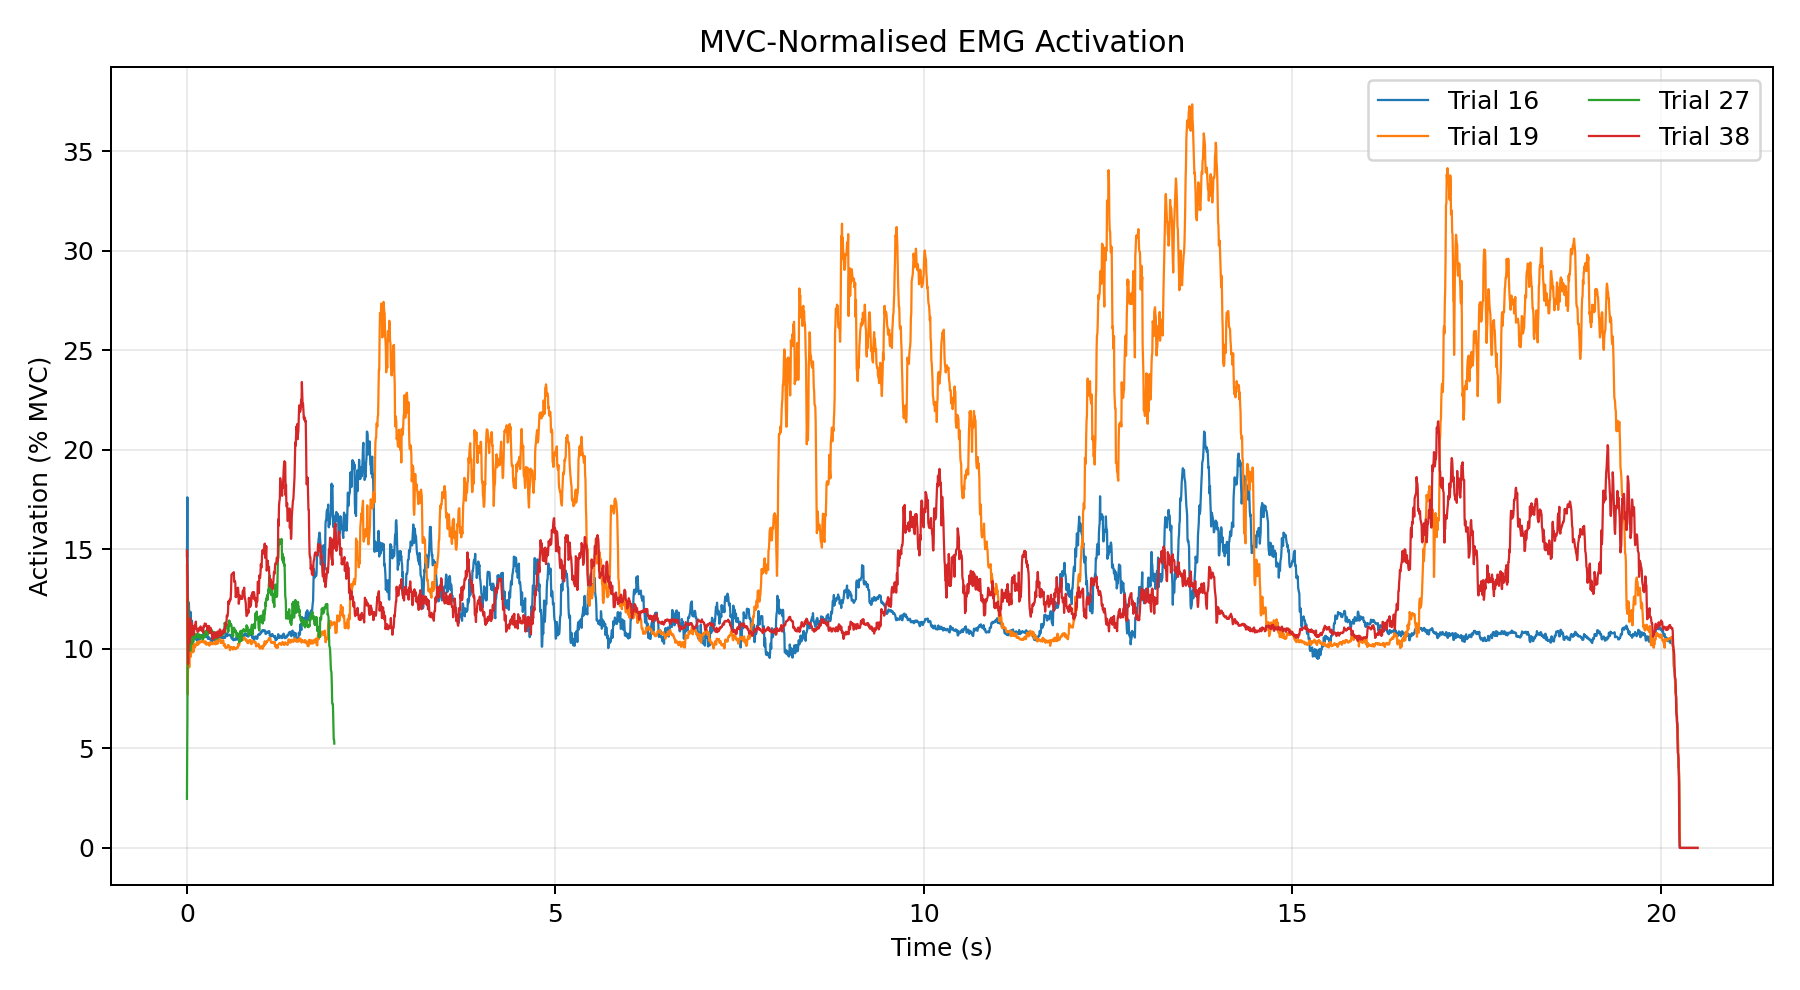
\includegraphics[width=0.95\textwidth]{emg_mvc_normalised_trials.png}
 \caption{Movement-trial RMS envelopes normalised to the peak MVC reference and expressed as percentage MVC.}
 \label{fig:mvc-normalised}
\end{figure}

\subsection{Interactive plots}
The raw, RMS, and MVC-normalised plots are provided in the companion HTML file
\csvfile{emg_report_interactive.html}. The page loads the renamed CSV files,
allows a trial to be selected, adjusts the RMS window, and switches between raw,
RMS, and normalised views. This supports the report figures by making the
processing steps reproducible from the exported data.

\section{Discussion}
The raw EMG trials show the direct sensor output and are most useful for
quality control. Large abrupt spikes or baseline shifts would indicate motion
artefact or poor electrode contact. A stable baseline and repeated activation
bursts indicate that the subject followed the motion instruction consistently.

RMS processing is required because EMG alternates rapidly around zero. Squaring
and averaging over a moving window produces a positive envelope that represents
local muscle activation. A shorter window follows rapid changes but remains
noisier; a longer window produces a smoother trace but can hide short bursts.
Therefore, the selected RMS window should be reported with the results.

MVC normalisation is important because raw EMG amplitude depends on electrode
placement, skin impedance, adipose tissue thickness, amplifier gain, and
subject-specific physiology. Dividing trial RMS by the MVC RMS reference
reduces these effects and presents activation as a percentage of the subject's
maximum recorded effort. This makes inter-trial and inter-subject comparisons
more meaningful, provided the MVC was performed correctly and without pain.

\section{Conclusion}
This practical recorded surface EMG data from EMG sensor 4, Channel 4, at
$4000\,\mathrm{Hz}$. The report uses four raw movement trials and one MVC
sliding-RMS file. Raw EMG is used to check signal quality and timing, RMS is
used to estimate the activation envelope, and MVC-normalised amplitude is used
to compare effort on a relative scale. The interactive HTML report provides the
required raw, RMS, and normalised graphs from the organised CSV files.

\end{document}
